\section{Architecture logique}
Frontend : le frontend est la partie visible de Vigilate, le site web.
Il est composé de plusieurs parties : paiement, paramétrage et alertes.
La partie paiement permet de souscrire aux abonnements proposés pour Vigilate.
La partie Paramétrage sert à spécifier quels programmes suivre et à partir de quelle criticité être avertie. Elle sert aussi à choisir par quel moyen être avertie.
La partie alerte prévient l'utilisateur s'il est affecté par une vulnérabilité.\\

Backend : le back-end est la face caché de Vigilate, il est en 2 parties : alerte et base de données.
La partie base de données stockera les programmes installés par les utilisateurs, leurs paramétrages ainsi que les vulnérabilités au fur et à mesure de leurs apparitions.
La partie alerte utilise cette base de données pour déterminer quels programmes sont vulnérable et avertir les utilisateurs par le moyen choisi. \\

Scanner de programme : le scanner de programme est un unique logiciel qui sert à récupérer la liste des programmes installés par un utilisateur. Il est donc composé de 3 parties : Linux, Windows, OSX.
Ces différentes parties font la même chose (recherche des programmes installés) mais chacune sur un système d'exploitation spécifique.\\

Api : l'api permet de lier tous les composants cités ci-dessus en leur permettant de communiquer et d'interagir entre eux. En plus de lier les composants, elle gérera les abonnements et sera disponible pour les revendeurs.
La partie abonnements de l'api s'occupera de permettre ou non aux utilisateurs d'utiliser Vigilate.
La partie revendeurs de l'api sera disponible afin de permettre une intégration facile de Vigilate dans des produits existant.
\newpage
\section{Flux et interactions}
Ci-dessous un schema explicatif de notre projet. On peut y voir chacun de nos modules ainsi que leurs intéractions, d'abord depuis notre serveur distant puis à partir d'une machine virtuelle. 
\begin{figure}[!h]
  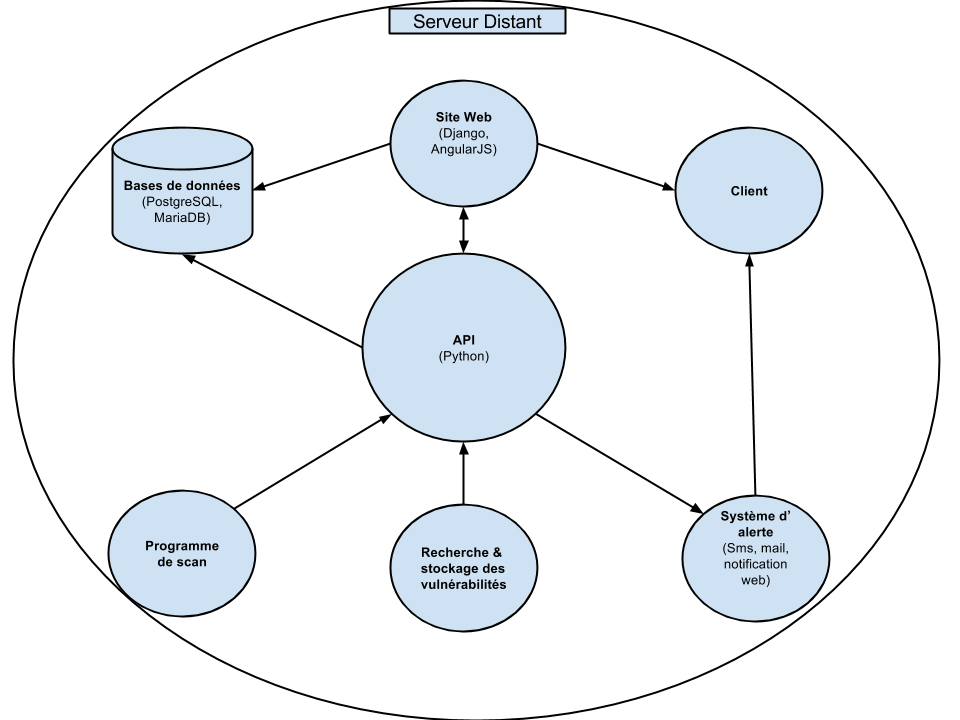
\includegraphics[width=18cm]{serveur-distant.png}
\end{figure}

\begin{figure}
  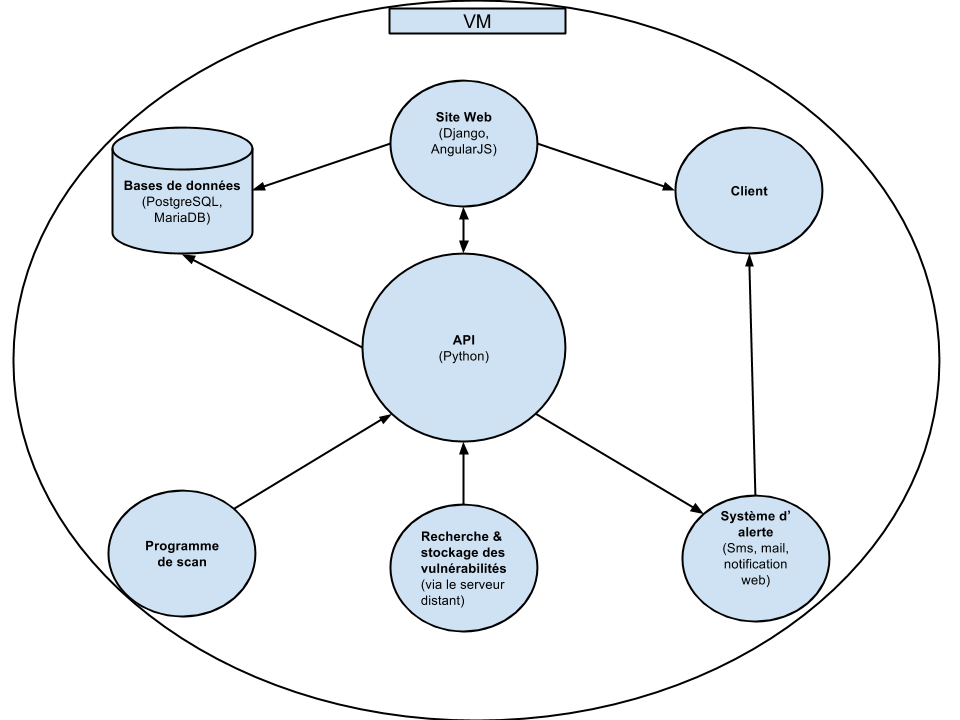
\includegraphics[width=18cm]{vm.png}
\end{figure}